\documentclass{standalone}
\usepackage{tikz}
\usetikzlibrary{patterns, positioning}
\usepackage[sfdefault]{ClearSans} %% option 'sfdefault' activates Clear Sans as the default text font
\usepackage[T1]{fontenc}

\begin{document}
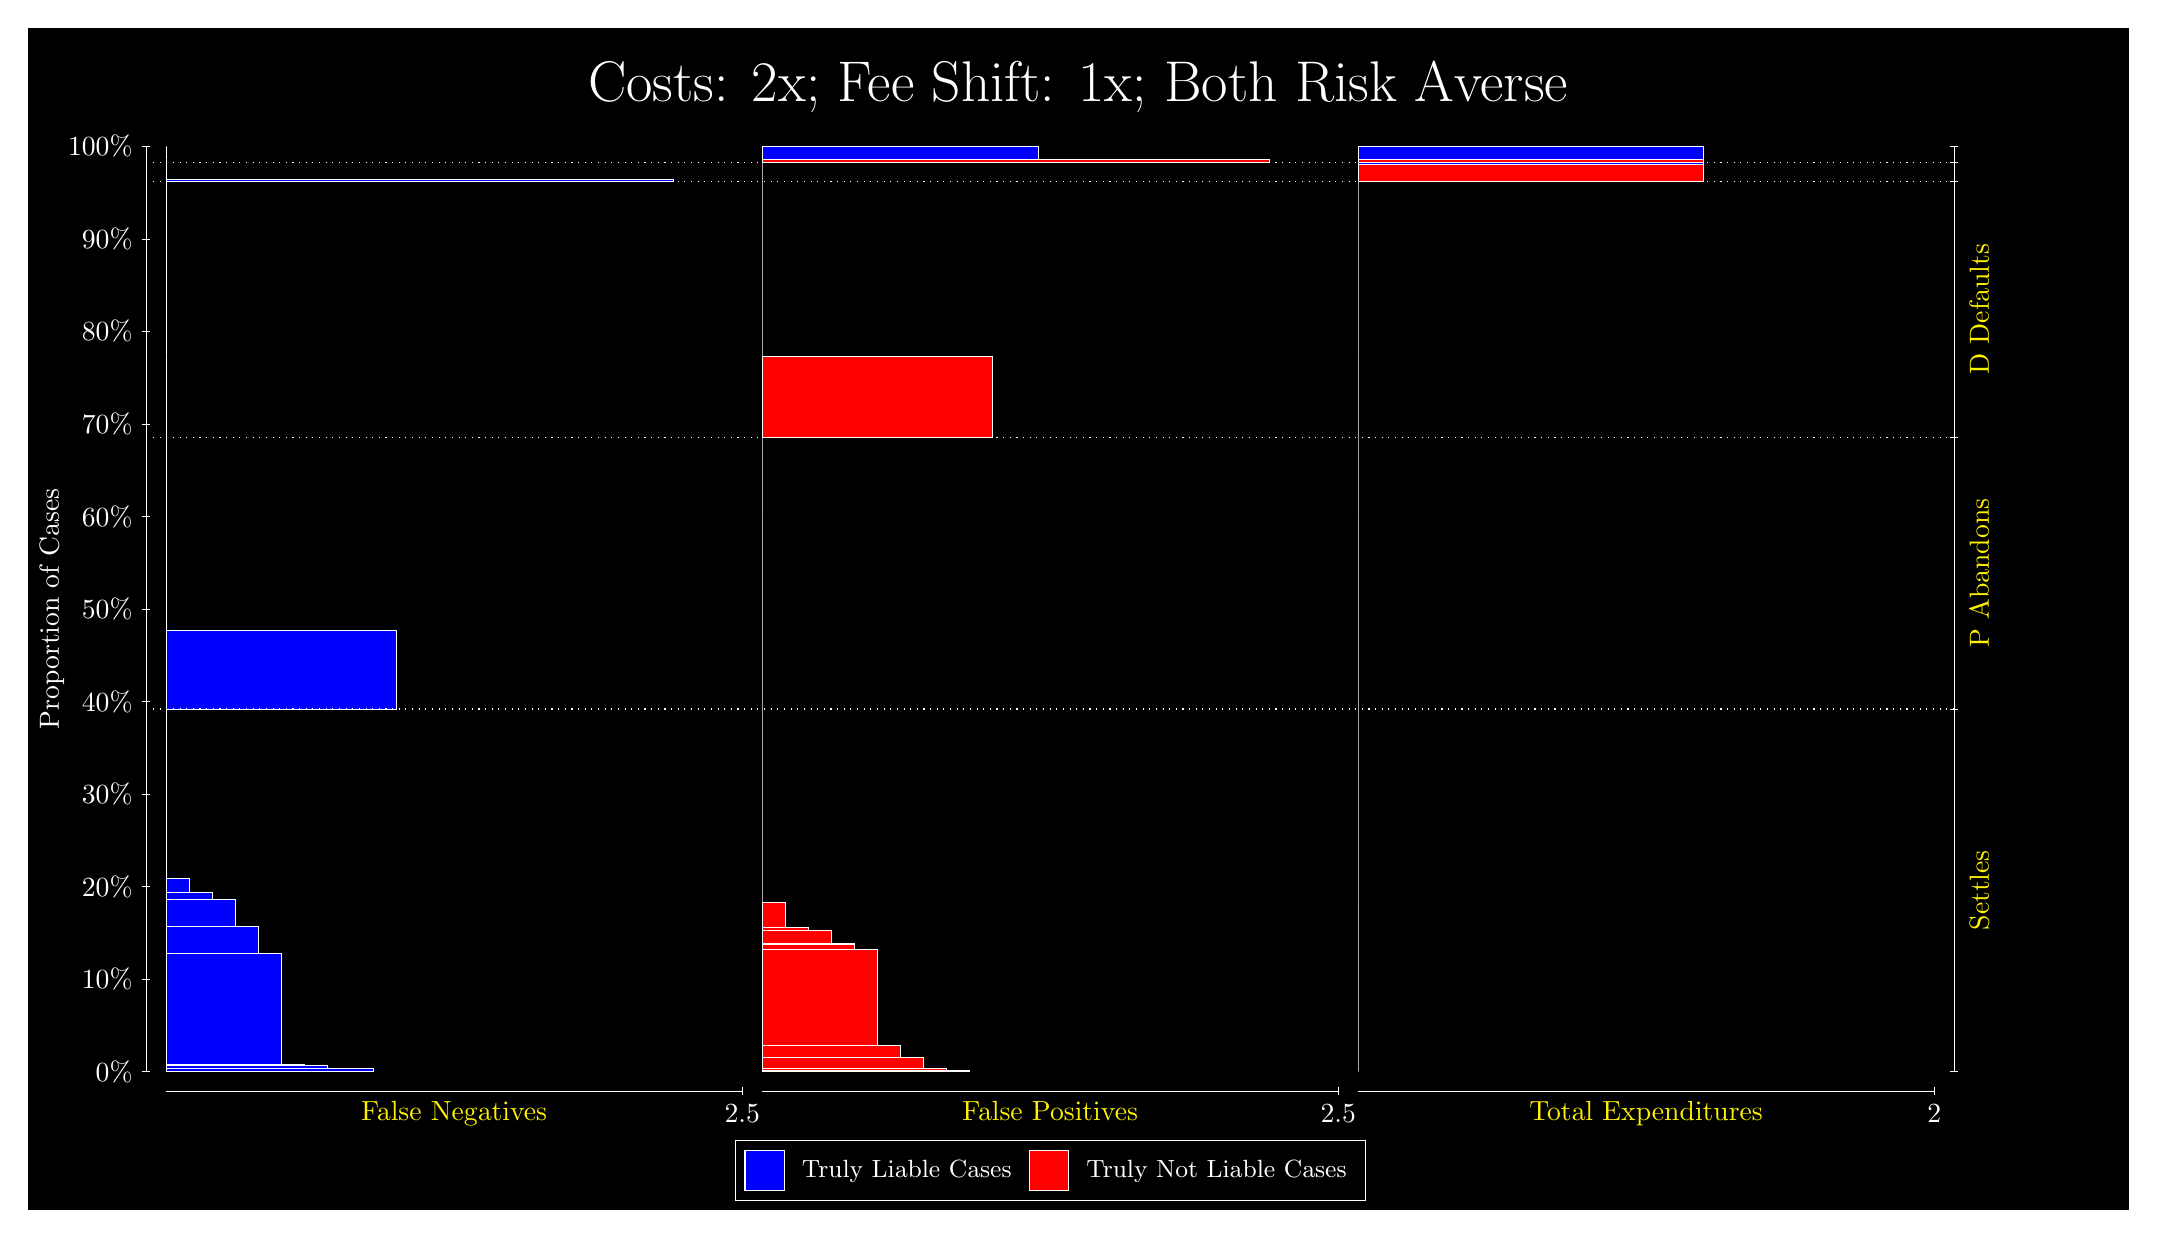
\begin{tikzpicture}
\draw[fill=black] (0,0) rectangle (26.667,15);
\draw[text=white] (0,13.5) rectangle (26.667,15) node[midway] {\huge Costs: 2x; Fee Shift: 1x; Both Risk Averse};
\draw[white, very thin] (1.5,1.75) -- (1.5,13.5);
\node[rotate=90, text=white, anchor=center] at (0.3, 7.625) {Proportion of Cases};
\draw[white, very thin] (1.45,1.75) -- (1.55,1.75);
\node[text=white, anchor=east] at (1.45, 1.75) {0\%};
\draw[white, very thin] (1.45,2.925) -- (1.55,2.925);
\node[text=white, anchor=east] at (1.45, 2.925) {10\%};
\draw[white, very thin] (1.45,4.1) -- (1.55,4.1);
\node[text=white, anchor=east] at (1.45, 4.1) {20\%};
\draw[white, very thin] (1.45,5.275) -- (1.55,5.275);
\node[text=white, anchor=east] at (1.45, 5.275) {30\%};
\draw[white, very thin] (1.45,6.45) -- (1.55,6.45);
\node[text=white, anchor=east] at (1.45, 6.45) {40\%};
\draw[white, very thin] (1.45,7.625) -- (1.55,7.625);
\node[text=white, anchor=east] at (1.45, 7.625) {50\%};
\draw[white, very thin] (1.45,8.8) -- (1.55,8.8);
\node[text=white, anchor=east] at (1.45, 8.8) {60\%};
\draw[white, very thin] (1.45,9.975) -- (1.55,9.975);
\node[text=white, anchor=east] at (1.45, 9.975) {70\%};
\draw[white, very thin] (1.45,11.15) -- (1.55,11.15);
\node[text=white, anchor=east] at (1.45, 11.15) {80\%};
\draw[white, very thin] (1.45,12.325) -- (1.55,12.325);
\node[text=white, anchor=east] at (1.45, 12.325) {90\%};
\draw[white, very thin] (1.45,13.5) -- (1.55,13.5);
\node[text=white, anchor=east] at (1.45, 13.5) {100\%};

\draw[white, very thin] (24.457,1.75) -- (24.457,13.5);
\draw[white, very thin] (24.407,1.75) -- (24.507,1.75);
\node[anchor=west] at (24.407, 1.75) {};
\draw[white, very thin] (24.407,6.3538) -- (24.507,6.3538);
\node[anchor=west] at (24.407, 6.3538) {};
\draw[white, very thin] (24.407,9.8069) -- (24.507,9.8069);
\node[anchor=west] at (24.407, 9.8069) {};
\draw[white, very thin] (24.407,13.057) -- (24.507,13.057);
\node[anchor=west] at (24.407, 13.057) {};
\draw[white, very thin] (24.407,13.3) -- (24.507,13.3);
\node[anchor=west] at (24.407, 13.3) {};
\draw[white, very thin] (24.407,13.5) -- (24.507,13.5);
\node[anchor=west] at (24.407, 13.5) {};

\draw[white, very thin, fill=blue] (1.75,1.75) rectangle (4.3848,1.7855);
\draw[white, very thin, fill=blue] (1.75,1.7855) rectangle (4.092,1.7892);
\draw[white, very thin, fill=blue] (1.75,1.7892) rectangle (3.7993,1.8278);
\draw[white, very thin, fill=blue] (1.75,1.8278) rectangle (3.5065,1.8336);
\draw[white, very thin, fill=blue] (1.75,1.8336) rectangle (3.5065,1.8455);
\draw[white, very thin, fill=blue] (1.75,1.8455) rectangle (3.2138,3.2515);
\draw[white, very thin, fill=blue] (1.75,3.2515) rectangle (2.921,3.5955);
\draw[white, very thin, fill=blue] (1.75,3.5955) rectangle (2.6283,3.9393);
\draw[white, very thin, fill=blue] (1.75,3.9393) rectangle (2.3355,4.0272);
\draw[white, very thin, fill=blue] (1.75,4.0272) rectangle (2.0428,4.2005);
\draw[white, very thin, fill=red] (1.75,4.2005) rectangle (1.75,6.3538);
\draw[white, very thin, fill=blue] (1.75,6.3538) rectangle (4.6775,7.3499);
\draw[white, very thin, fill=red] (1.75,7.3499) rectangle (1.75,9.8069);
\draw[white, very thin, fill=red] (1.75,9.8069) rectangle (1.75,10.829);
\draw[white, very thin, fill=blue] (1.75,10.829) rectangle (1.75,13.057);
\draw[white, very thin, fill=blue] (1.75,13.057) rectangle (8.1906,13.087);
\draw[white, very thin, fill=red] (1.75,13.087) rectangle (1.75,13.3);
\draw[white, very thin, fill=red] (1.75,13.3) rectangle (1.75,13.33);
\draw[white, very thin, fill=blue] (1.75,13.33) rectangle (1.75,13.5);
\draw[white, very thin, fill=red] (9.3189,1.75) rectangle (11.954,1.7655);
\draw[white, very thin, fill=red] (9.3189,1.7655) rectangle (11.661,1.7928);
\draw[white, very thin, fill=red] (9.3189,1.7928) rectangle (11.368,1.9254);
\draw[white, very thin, fill=red] (9.3189,1.9254) rectangle (11.075,2.08);
\draw[white, very thin, fill=red] (9.3189,2.08) rectangle (10.783,3.3057);
\draw[white, very thin, fill=red] (9.3189,3.3057) rectangle (10.49,3.3614);
\draw[white, very thin, fill=red] (9.3189,3.3614) rectangle (10.49,3.3748);
\draw[white, very thin, fill=red] (9.3189,3.3748) rectangle (10.197,3.5456);
\draw[white, very thin, fill=red] (9.3189,3.5456) rectangle (9.9044,3.5849);
\draw[white, very thin, fill=red] (9.3189,3.5849) rectangle (9.6116,3.9033);
\draw[white, very thin, fill=blue] (9.3189,3.9033) rectangle (9.3189,6.3538);
\draw[white, very thin, fill=red] (9.3189,6.3538) rectangle (9.3189,8.8109);
\draw[white, very thin, fill=blue] (9.3189,8.8109) rectangle (9.3189,9.8069);
\draw[white, very thin, fill=red] (9.3189,9.8069) rectangle (12.246,10.829);
\draw[white, very thin, fill=blue] (9.3189,10.829) rectangle (9.3189,13.057);
\draw[white, very thin, fill=red] (9.3189,13.057) rectangle (9.3189,13.27);
\draw[white, very thin, fill=blue] (9.3189,13.27) rectangle (9.3189,13.3);
\draw[white, very thin, fill=red] (9.3189,13.3) rectangle (15.759,13.33);
\draw[white, very thin, fill=blue] (9.3189,13.33) rectangle (12.832,13.5);
\draw[white, very thin, fill=red] (16.888,1.75) rectangle (16.888,3.9033);
\draw[white, very thin, fill=blue] (16.888,3.9033) rectangle (16.888,6.3538);
\draw[white, very thin, fill=red] (16.888,6.3538) rectangle (16.888,8.8109);
\draw[white, very thin, fill=blue] (16.888,8.8109) rectangle (16.888,9.8069);
\draw[white, very thin, fill=red] (16.888,9.8069) rectangle (16.888,10.829);
\draw[white, very thin, fill=blue] (16.888,10.829) rectangle (16.888,13.057);
\draw[white, very thin, fill=red] (16.888,13.057) rectangle (21.279,13.27);
\draw[white, very thin, fill=blue] (16.888,13.27) rectangle (21.279,13.3);
\draw[white, very thin, fill=red] (16.888,13.3) rectangle (21.279,13.33);
\draw[white, very thin, fill=blue] (16.888,13.33) rectangle (21.279,13.5);
\draw[white, dotted] (1.5,6.3538) -- (24.457,6.3538);
\draw[white, dotted] (1.5,9.8069) -- (24.457,9.8069);
\draw[white, dotted] (1.5,13.057) -- (24.457,13.057);
\draw[white, dotted] (1.5,13.3) -- (24.457,13.3);
\draw[white, very thin] (1.75,1.5) -- (9.0689,1.5);
\node[text=yellow, anchor=north] at (5.4094, 1.5) {False Negatives};
\draw[white, very thin] (9.0689,1.45) -- (9.0689,1.55);
\node[text=white, anchor=north] at (9.0689, 1.45) {2.5};

\draw[white, very thin] (9.3189,1.5) -- (16.638,1.5);
\node[text=yellow, anchor=north] at (12.978, 1.5) {False Positives};
\draw[white, very thin] (16.638,1.45) -- (16.638,1.55);
\node[text=white, anchor=north] at (16.638, 1.45) {2.5};

\draw[white, very thin] (16.888,1.5) -- (24.207,1.5);
\node[text=yellow, anchor=north] at (20.547, 1.5) {Total Expenditures};
\draw[white, very thin] (24.207,1.45) -- (24.207,1.55);
\node[text=white, anchor=north] at (24.207, 1.45) {2};

\node[text=yellow, centered, rotate=90] at (24.777, 4.0519) {Settles};
\node[text=yellow, centered, rotate=90] at (24.777, 8.0804) {P Abandons};
\node[text=yellow, centered, rotate=90] at (24.777, 11.432) {D Defaults};



\draw (12.978300999999998,1.5) node[draw=none] (baseCoordinate) {};
\begin{scope}[align=center]
        \matrix[scale=0.5, draw=white, below=0.5cm of baseCoordinate, nodes={draw}, column sep=0.1cm]{
            \node[rectangle, draw, minimum width=0.5cm, minimum height=0.5cm, fill=blue] {}; &
            \node[draw=none, font=\small, text=white] (B) {Truly Liable Cases}; &
            \node[rectangle, draw, minimum width=0.5cm, minimum height=0.5cm, fill=red] {}; &
            \node[draw=none, font=\small, text=white] (B) {Truly Not Liable Cases}; \\
            };
\end{scope}

\end{tikzpicture}
\end{document}